\documentclass[12pt, titlepage]{article}

\usepackage{fullpage}
\usepackage[round]{natbib}
\usepackage{multirow}
\usepackage{booktabs}
\usepackage{tabularx}
\usepackage{graphicx}
\usepackage{float}
\usepackage{hyperref}
\hypersetup{
    colorlinks,
    citecolor=blue,
    filecolor=black,
    linkcolor=red,
    urlcolor=blue
}

\input{../../Comments}
\input{../../Common}

\newcounter{acnum}
\newcommand{\actheacnum}{AC\theacnum}
\newcommand{\acref}[1]{AC\ref{#1}}

\newcounter{ucnum}
\newcommand{\uctheucnum}{UC\theucnum}
\newcommand{\uref}[1]{UC\ref{#1}}

\newcounter{mnum}
\newcommand{\mthemnum}{M\themnum}
\newcommand{\mref}[1]{M\ref{#1}}

\begin{document}

\title{Module Guide for \progname{}} 
\author{\authname}
\date{\today}

\maketitle

\pagenumbering{roman}

\section{Revision History}

\begin{tabularx}{\textwidth}{p{3cm}p{2cm}X}
\toprule {\bf Date} & {\bf Version} & {\bf Notes}\\
\midrule
January 13, 2025 & 1.0 & TA Feedback\\
January 17, 2025 & 1.1 & Rev0\\
April 1, 2025 & 1.2 & Based on TA feedback: Exact appendix referenced in
section 10. Changed sections 7.1 and 7.2 titles to be grammatically correct.
Season scheduler module is a SW decision module as it can be replaced with
different scheduling algorithms.\\
April 2, 2025 & 1.3 & Based on TA feedback: References seem to be working
appropriately.\\
April 4, 2025 & 1.4 & Updated names of 'structure' modules to 'record modules' to match new hierarchy diagram.
Based on TA feedback: Changed use hierarchy diagram and appendix screenshots to PDF from image.\\
\bottomrule
\end{tabularx}

\newpage

\section{Reference Material}

This section records information for easy reference.

\subsection{Abbreviations and Acronyms}

\renewcommand{\arraystretch}{1.2}
\begin{tabular}{l l} 
  \toprule		
  \textbf{symbol} & \textbf{description}\\
  \midrule 
  AC & Anticipated Change\\
  DAG & Directed Acyclic Graph \\
  M & Module \\
  MG & Module Guide \\
  OS & Operating System \\
  R & Requirement\\
  SC & Scientific Computing \\
  SRS & Software Requirements Specification\\
  \progname & Explanation of program name\\
  UC & Unlikely Change \\
  \bottomrule
\end{tabular}\\

\newpage

\tableofcontents

\listoftables

\listoffigures

\newpage

\pagenumbering{arabic}

\section{Introduction}

Decomposing a system into modules is a commonly accepted approach to developing
software.  A module is a work assignment for a programmer or programming
team~\citep{ParnasEtAl1984}.  We advocate a decomposition
based on the principle of information hiding~\citep{Parnas1972a}.  This
principle supports design for change, because the ``secrets'' that each module
hides represent likely future changes.  Design for change is valuable in SC,
where modifications are frequent, especially during initial development as the
solution space is explored.  

Our design follows the rules layed out by \citet{ParnasEtAl1984}, as follows:
\begin{itemize}
\item System details that are likely to change independently should be the
  secrets of separate modules.
\item Each data structure is implemented in only one module as a 'record module'.
\item Any other program that requires information stored in a module's data
  structures must obtain it by calling access programs belonging to that module.
\end{itemize}

After completing the first stage of the design, the Software Requirements
Specification (SRS), the Module Guide (MG) is developed~\citep{ParnasEtAl1984}. The MG
specifies the modular structure of the system and is intended to allow both
designers and maintainers to easily identify the parts of the software.  The
potential readers of this document are as follows:

\begin{itemize}
\item New project members: This document can be a guide for a new project member
  to easily understand the overall structure and quickly find the
  relevant modules they are searching for.
\item Maintainers: The hierarchical structure of the module guide improves the
  maintainers' understanding when they need to make changes to the system. It is
  important for a maintainer to update the relevant sections of the document
  after changes have been made.
\item Designers: Once the module guide has been written, it can be used to
  check for consistency, feasibility, and flexibility. Designers can verify the
  system in various ways, such as consistency among modules, feasibility of the
  decomposition, and flexibility of the design.
\end{itemize}

The rest of the document is organized as follows. Section
\ref{SecChange} lists the anticipated and unlikely changes of the software
requirements. Section \ref{SecMH} summarizes the module decomposition that
was constructed according to the likely changes. Section \ref{SecConnection}
specifies the connections between the software requirements and the
modules. Section \ref{SecMD} gives a detailed description of the
modules. Section \ref{SecTM} includes two traceability matrices. One checks
the completeness of the design against the requirements provided in the SRS. The
other shows the relation between anticipated changes and the modules. Section
\ref{SecUse} describes the use relation between modules.

\section{Anticipated and Unlikely Changes} \label{SecChange}

This section lists possible changes to the system. According to the likeliness
of the change, the possible changes are classified into two
categories. Anticipated changes are listed in Section \ref{SecAchange}, and
unlikely changes are listed in Section \ref{SecUchange}.

\subsection{Anticipated Changes} \label{SecAchange}

Anticipated changes are the source of the information that is to be hidden
inside the modules. Ideally, changing one of the anticipated changes will only
require changing the one module that hides the associated decision. The approach
adapted here is called design for
change.

\begin{description}
  \item[\refstepcounter{acnum} \actheacnum \label{acHardware}:] The specific
  hardware on which the software is running.
  \item[\refstepcounter{acnum} \actheacnum \label{acLogIn}:] The format of the
  log in process and data.
  \item[\refstepcounter{acnum} \actheacnum \label{acSched}:] The algorithm
  used for the season scheduler.
  \item[\refstepcounter{acnum} \actheacnum \label{acSchedConstraints}:] The
  constraints on the season schedule.
  \item[\refstepcounter{acnum} \actheacnum \label{acAvailability}:] The format
  of a team's season availability data.
  \item[\refstepcounter{acnum} \actheacnum \label{acSchedConflicts}:] How
  scheduling conflicts are to be resolved.
  \item[\refstepcounter{acnum} \actheacnum \label{acSchedFormat}:] The format
  of the season schedule.
  \item[\refstepcounter{acnum} \actheacnum \label{acCreateAccount}:] The
  format of the create player/team account process and data.
  \item[\refstepcounter{acnum} \actheacnum \label{acJoinRequest}:] The process
  of a player requesting to join a team.
  \item[\refstepcounter{acnum} \actheacnum \label{acAdmin}:] The process of a
  commissioner making an admin command.
  \item[\refstepcounter{acnum} \actheacnum \label{acAlertSend}:] The process
  of creating an alert.
  \item[\refstepcounter{acnum} \actheacnum \label{acReschedule}:] The process
  of rescheduling a game.
  \item[\refstepcounter{acnum} \actheacnum \label{acAlertReceive}:] The method
  by which alerts are received.
\end{description}

\subsection{Unlikely Changes} \label{SecUchange}

The module design should be as general as possible. However, a general system is
more complex. Sometimes this complexity is not necessary. Fixing some design
decisions at the system architecture stage can simplify the software design. If
these decision should later need to be changed, then many parts of the design
will potentially need to be modified. Hence, it is not intended that these
decisions will be changed.

\begin{description}
  \item[\refstepcounter{ucnum} \uctheucnum \label{ucIO}:] Input/Output devices
  (Input: File and/or Keyboard, Output: File, Memory, and/or Screen).
  \item[\refstepcounter{ucnum} \uctheucnum \label{ucWeb}:] The system being a
  web application.
  \item[\refstepcounter{ucnum} \uctheucnum \label{ucAccStr}:] Player, team,
  and commissioner account records.
  \item[\refstepcounter{ucnum} \uctheucnum \label{ucSched}:] The goal of the
  system to generate a season schedule.
\end{description}

\section{Module Hierarchy} \label{SecMH}

This section provides an overview of the module design. Modules are summarized
in a hierarchy decomposed by secrets in Table \ref{TblMH}. The modules listed
below, which are leaves in the hierarchy tree, are the modules that will
be implemented.

\begin{description}
  \item [\refstepcounter{mnum} \mthemnum \label{mHH}:] Hardware Hiding Module
  \item [\refstepcounter{mnum} \mthemnum \label{mAC}:] Account Module
  \item [\refstepcounter{mnum} \mthemnum \label{mPL}:] Player Module
  \item [\refstepcounter{mnum} \mthemnum \label{mTE}:] Team Module
  \item [\refstepcounter{mnum} \mthemnum \label{mCM}:] Commissioner Module
  \item [\refstepcounter{mnum} \mthemnum \label{mAS}:] Account Records
  Module
  \item [\refstepcounter{mnum} \mthemnum \label{mTS}:] Team Records Module
  \item [\refstepcounter{mnum} \mthemnum \label{mSS}:] Schedule Records
  Module
  \item [\refstepcounter{mnum} \mthemnum \label{mS}:] Season Scheduler Module
  \item [\refstepcounter{mnum} \mthemnum \label{mRE}:] Reschedule Module
  \item [\refstepcounter{mnum} \mthemnum \label{mAL}:] Alerts Module
  \item [\refstepcounter{mnum} \mthemnum \label{mDB}:] Database Module
\end{description}


\begin{table}[h!]
\centering
\begin{tabular}{p{0.3\textwidth} p{0.6\textwidth}}
\toprule
\textbf{Level 1} & \textbf{Level 2}\\
\midrule

{Hardware-Hiding Module} & ~ \\
\midrule

\multirow{11}{0.3\textwidth}{Behaviour-Hiding Module} & Account Module\\
& Player Module\\
& Team Module\\
& Commissioner Module\\
& Account Records Module\\
& Team Records Module\\
& Schedule Records Module\\
& Reschedule Module\\
& Alerts Module\\
& Database Module\\
\midrule

{Software Decision Module} & Season Scheduler
Module\\
\midrule

\end{tabular}
\caption{Module Hierarchy}
\label{TblMH}
\end{table}

\section{Connection Between Requirements and Design} \label{SecConnection}

The design of the system is intended to satisfy the requirements developed in
the SRS. In this stage, the system is decomposed into modules. The connection
between requirements and modules is listed in Table~\ref{TblRT}.

\section{Module Decomposition} \label{SecMD}

Modules are decomposed according to the principle of ``information hiding''
proposed by \citet{ParnasEtAl1984}. The \emph{Secrets} field in a module
decomposition is a brief statement of the design decision hidden by the
module. The \emph{Services} field specifies \emph{what} the module will do
without documenting \emph{how} to do it. For each module, a suggestion for the
implementing software is given under the \emph{Implemented By} title. If the
entry is \emph{OS}, this means that the module is provided by the operating
system or by standard programming language libraries.  \emph{\progname{}}
means the module will be implemented by the \progname{} software.

Only the leaf modules in the hierarchy have to be implemented. If a dash
(\emph{--}) is shown, this means that the module is not a leaf and will not
have to be implemented.

\subsection{Hardware Hiding Module (\mref{mHH})}

\begin{description}
  \item[Secrets:]The data structure and algorithm used to implement the
  virtual hardware.
  \item[Services:]Serves as a virtual hardware used by the rest of the
  system. This module provides the interface between the hardware and the
  software. So, the system can use it to display outputs or to accept inputs.
  \item[Implemented By:] OS
\end{description}

\subsection{Behaviour-Hiding Modules}

\begin{description}
  \item[Secrets:]The contents of the required behaviours.
  \item[Services:]Includes programs that provide externally visible behaviour
  of the system as specified in the software requirements specification (SRS)
  documents. This module serves as a communication layer between the
  hardware-hiding module and the software decision module. The programs in
  this module will need to change if there are changes in the SRS.
  \item[Implemented By:] --
\end{description}

\subsubsection{Account Module (\mref{mAC})}

\begin{description}
  \item[Secrets:]The general functionality of all accounts.
  \item[Services:]Contains functions to allow the user to create, delete,
  login, and edit their \progname{} account.
  \item[Implemented By:] \progname{}
  \item[Type of Module:] Abstract Object
\end{description}

\subsubsection{Player Module (\mref{mPL})}

\begin{description}
  \item[Secrets:]The functionality of a player account.
  \item[Services:]Contains functions to allow the user to join and leave a
  team.
  \item[Implemented By:] \progname{}
  \item[Type of Module:] Abstract Object
\end{description}

\subsubsection{Team Module (\mref{mTE})}

\begin{description}
  \item[Secrets:]The functionality of a team account.
  \item[Services:]Contains functions to allow the user to submit a game score
  and access to the Reschedule Module functionality.
  \item[Implemented By:] \progname{}
  \item[Type of Module:] Abstract Object
\end{description}

\subsubsection{Commissioner Module (\mref{mCM})}

\begin{description}
  \item[Secrets:]The functionality of a commissioner account.
  \item[Services:]Contains functions to allow the user to perform defined
  admin commands and send alerts.
  \item[Implemented By:] \progname{}
  \item[Type of Module:] Abstract Object
\end{description}

\subsubsection{Account Records Module (\mref{mAS})}

\begin{description}
  \item[Secrets:]The format of the account data.
  \item[Services:]Defines a general account data structure for all accounts,
  including player, team, and commissioner accounts.
  \item[Implemented By:] \progname{}
  \item[Type of Module:] Abstract Data Type
\end{description}

\subsubsection{Team Records Module (\mref{mTS})}

\begin{description}
  \item[Secrets:]The format of the team account data.
  \item[Services:]Defines a team account data records that inherits from the
  account records module.
  \item[Implemented By:] \progname{}
  \item[Type of Module:] Abstract Data Type
\end{description}

\subsubsection{Schedule Records Module (\mref{mSS})}

\begin{description}
  \item[Secrets:]The format of the season schedule data.
  \item[Services:]Defines a season schedule data structure.
  \item[Implemented By:] \progname{}
  \item[Type of Module:] Abstract Data Type
\end{description}

\subsubsection{Reschedule Module (\mref{mRE})}

\begin{description}
  \item[Secrets:]The function of a team account to request and accept a game
  reschedule.
  \item[Services:]Contains functions to allow the user to request and accept a
  game reschedule.
  \item[Implemented By:] \progname{}
  \item[Type of Module:] Library
\end{description}

\subsubsection{Alerts Module (\mref{mAL})}

\begin{description}
  \item[Secrets:]The function of a commissioner account to create and send
  alerts.
  \item[Services:]Contains functions to allow the user to create and send alerts.
  \item[Implemented By:] \progname{}
  \item[Type of Module:] Library
\end{description}

\subsubsection{Database Module (\mref{mDB})}

\begin{description}
  \item[Secrets:]The function of storing player, team, commissioner, and schedule data.
  \item[Services:]Defines and maintains a database that stores all relevant data
  to the \progname{} system. This includes account data for players, teams, and
  commissioners such as contact information and team player lists. It also
  includes full game lists for the schedule and game scores. The maintenance
  includes regular backups and data integrity checks.
  \item[Implemented By:] \progname{}
  \item[Type of Module:] Library
\end{description}


\subsection{Software Decision Module}

\begin{description}
  \item[Secrets:] The design decision based on mathematical theorems, physical
  facts, or programming considerations. The secrets of this module are
  \emph{not} described in the SRS.
  \item[Services:] Includes data structure and algorithms used in the system that
  do not provide direct interaction with the user. 
  % Changes in these modules are more likely to be motivated by a desire to
  % improve performance than by externally imposed changes.
  \item[Implemented By:] --
\end{description}

\subsubsection{Season Scheduler Module (\mref{mS})}

\begin{description}
  \item[Secrets:]The algorithm used to generate a season schedule.
  \item[Services:]The algorithm generates a season schedule using each teams
  availability and a set of constraints as inputs and outputs a schedule of
  the form of the data structure defined in the schedule records module.
  \item[Implemented By:] \progname{}
\end{description}

\section{Traceability Matrix} \label{SecTM}

This section shows two traceability matrices: between the modules and the
requirements and between the modules and the anticipated changes.

% the table should use mref, the requirements should be named, use something
% like fref
\begin{table}[H]
\centering
\begin{tabular}{p{0.2\textwidth} p{0.6\textwidth}}
\toprule
\textbf{Req.} & \textbf{Modules}\\
\midrule
FR-1 & \mref{mST}, \mref{mS},\\
FR-2 & \mref{mTE}, \mref{mDB}\\
FR-3 & \mref{mAC}, \mref{mAS}\\
FR-4 & \mref{mAC}, \mref{mAS}\\
FR-5 & \mref{mAC}, \mref{mAS}\\
FR-6 & \mref{mCM}, \mref{mAL}\\
FR-7 & \mref{mTE}, \mref{mCM}\\
FR-8 & \mref{mPL},\\
FR-9 & \mref{mS}\\
FR-10 & \mref{mPL}, \mref{mRE}\\
FR-11 & \mref{mPL}, \mref{mRE}\\
FR-12 & \mref{mPL}, \mref{mRE}\\
FR-13 & \mref{mPL}, \mref{mTE}\\
FR-14 & \mref{mPL}, \mref{mTE}\\
FR-15 & \mref{mPL}, \mref{mTE}\\
FR-16 & \mref{mAC}\\
FR-17 & \mref{mPL}, \mref{mTE}\\
FR-18 & \mref{mCM}, \mref{mS}\\
FR-19 & \mref{mPL}, \mref{mCM}, \mref{mTS}\\
FR-20 & \mref{mSS}, \mref{mS}\\
FR-21 & \mref{mTS}, \mref{mSS}, \mref{mS}\\
FR-22 & \mref{mCM}, \mref{mSS}, \mref{mS}\\
FR-23 & \mref{mTS}\\
FR-24 & \mref{mAC}\\
\bottomrule
\end{tabular}
\caption{Trace Between Functional Requirements and Modules}
\label{TblRT}
\end{table}

\begin{table}[H]
\centering
\begin{tabular}{p{0.2\textwidth} p{0.6\textwidth}}
\toprule
\textbf{AC} & \textbf{Modules}\\
\midrule
\acref{acHardware} & \mref{mHH}\\
\acref{acLogIn} & \mref{mAC}, \mref{mAS}, \mref{mDB}\\
\acref{acSched} & \mref{mS}\\
\acref{acSchedConstraints} & \mref{mSS}\\
\acref{acAvailability} & \mref{mPL}, \mref{mDB}\\
\acref{acSchedConflicts} & \mref{mSS}\\
\acref{acSchedFormat} & \mref{mSS}\\
\acref{acStandFormat} & \mref{mST}\\
\acref{acCreateAccount} & \mref{mPL}, \mref{mTE}, \mref{mDB}\\
\acref{acJoinRequest} & \mref{mPL}, \mref{mTE}\\
\acref{acAdmin} & \mref{mCM}\\
\acref{acAlertSend} & \mref{mAL}\\
\acref{acReschedule} & \mref{mPL}, \mref{mRE}\\
\acref{acAlertReceive} & \mref{mAL}\\
\bottomrule
\end{tabular}
\caption{Trace Between Anticipated Changes and Modules}
\label{TblACT}
\end{table}

\section{Use Hierarchy Between Modules} \label{SecUse}

In this section, the uses hierarchy between modules is
provided. \citet{Parnas1978} said of two programs A and B that A {\em uses} B if
correct execution of B may be necessary for A to complete the task described in
its specification. That is, A {\em uses} B if there exist situations in which
the correct functioning of A depends upon the availability of a correct
implementation of B.  Figure \ref{FigUH} illustrates the use relation between
the modules. It can be seen that the graph is a directed acyclic graph
(DAG). Each level of the hierarchy offers a testable and usable subset of the
system, and modules in the higher level of the hierarchy are essentially simpler
because they use modules from the lower levels.

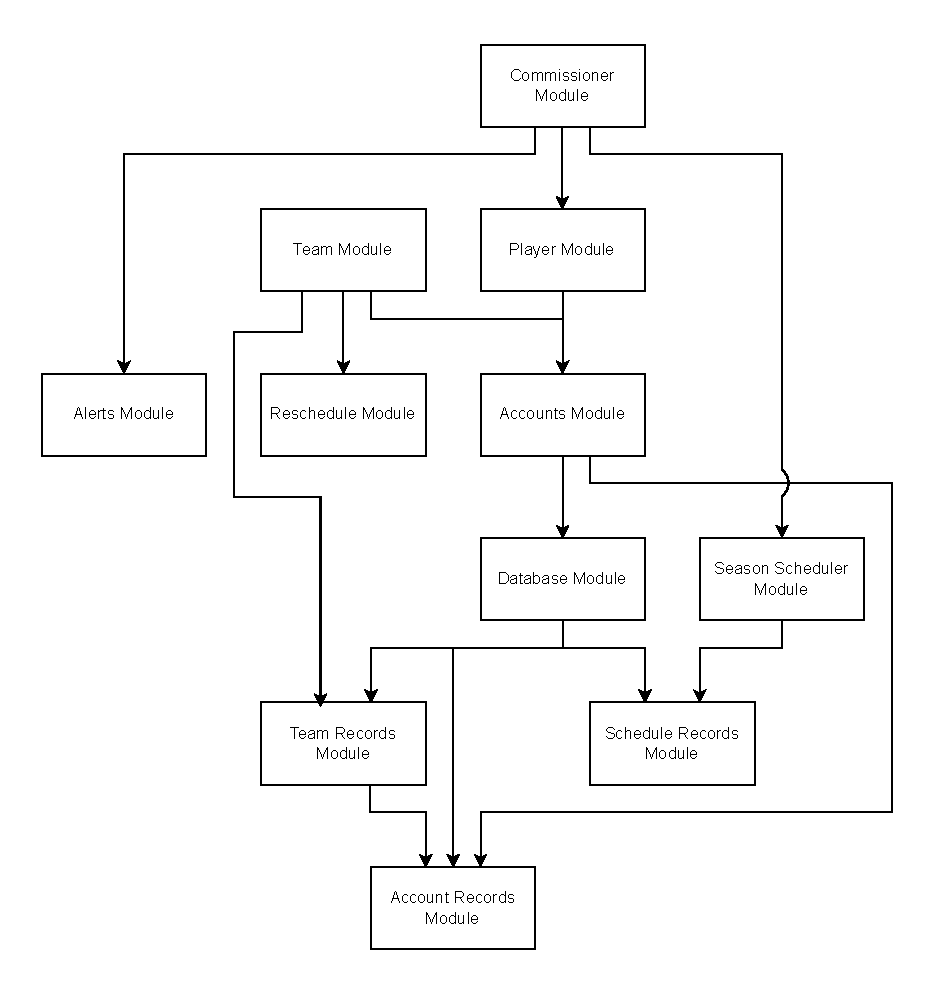
\includegraphics[scale=1]{9_use_hierarchy_diagram.pdf}

\begin{figure}[H]
\centering
%\includegraphics[width=0.7\textwidth]{UsesHierarchy.png}
\caption{Use hierarchy among modules}
\label{FigUH}
\end{figure}

%\section*{References}

\section{User Interfaces}

Preliminary design of the major user interfaces can be found in the \href{https://www.figma.com/proto/5YNR4bBk1vqGhvvdioqJnI/Capstone-MG-Sketches?node-id=4-2&p=f&t=sLgjpB9bWIdGXPd8-1&scaling=scale-down&content-scaling=fixed&page-id=0%3A1}{Figma}.
Screens are also provided in the \nameref{Appendix}.

\section{Design of Communication Protocols}

The design of the communication protocols define how the modules will interact within the system.
where the system will use both synchronous (for real-time interactions like user authentication)
and asynchronous (for background operations like logging) communication methods.
Key technologies will include HTTP/HTTPS for secure data transmission, REST APIs for
resource access, WebSockets for real-time updates, and message queues (e.g., RabbitMQ)
for asynchronous communication. Data formats used are JSON for lightweight data exchange
and XML for structured configuration files. Robust communication is ensured through error
handling and retry mechanisms, managing issues like network failures and invalid data.
Security measures include authentication and authorization using tokens (e.g., JWT) and
encryption via HTTPS. For example, a POST request may be sent by a user to create an account,
where the Account Module would process and store the data, responding with a corresponding account ID.

\section{Timeline}

The implementation of modules for Rev 0 will follow the detailed timeline below.
Daily stand-up meetings will be held to track each team member's progress and address
any issues they may have run into, prior to the meeting. Each module will have unit
tests to ensure successful functionality, and integration tests will be performed
after integrating each module. Final testing will then validate the core functionality,
making sure the performance of the system is able to accomplish each module's functions.

\begin{itemize}
  \item \textbf{Week 1 (January 13-19)}: Initial Setup and Planning
    \begin{itemize}
      \item Create Github issues that team members will assign themselves
      (All team members)
    \end{itemize}
  \item \textbf{Week 2 (January 20-26)}: Core Module Implementation
    \begin{itemize}
      \item Implement the account module (Casra Ghazanfari)
      \item Implement the player, team, and commissioner modules (Nicholas Fabugais-Inaba)
      \item Setup database module for storing different data (Casra Ghazanfari)
      \item Create the schedule record modules (Jung Woo Lee)
      \item Update season scheduler module to generate an optimal schedule (Alex Verity)
    \end{itemize}
  \item \textbf{Week 3 (January 27-February 2)}: Remaining Modules and Integration
    \begin{itemize}
      \item Implement alerts module (Alex Verity)
      \item Implement reschedule module (Jung Woo Lee)
      \item Initial integration testing (All team members)
    \end{itemize}
  \item \textbf{Week 4 (February 3)}: Final Integration and Testing
    \begin{itemize}
      \item Design and implement the user interface (Nicholas Fabugais-Inaba)
      \item Final integration and comprehensive testing (All team members)
    \end{itemize}
\end{itemize}

\bibliographystyle {plainnat}
\bibliography{../../../refs/References}

\newpage{}

\section{Appendix} \label{Appendix}

\centering
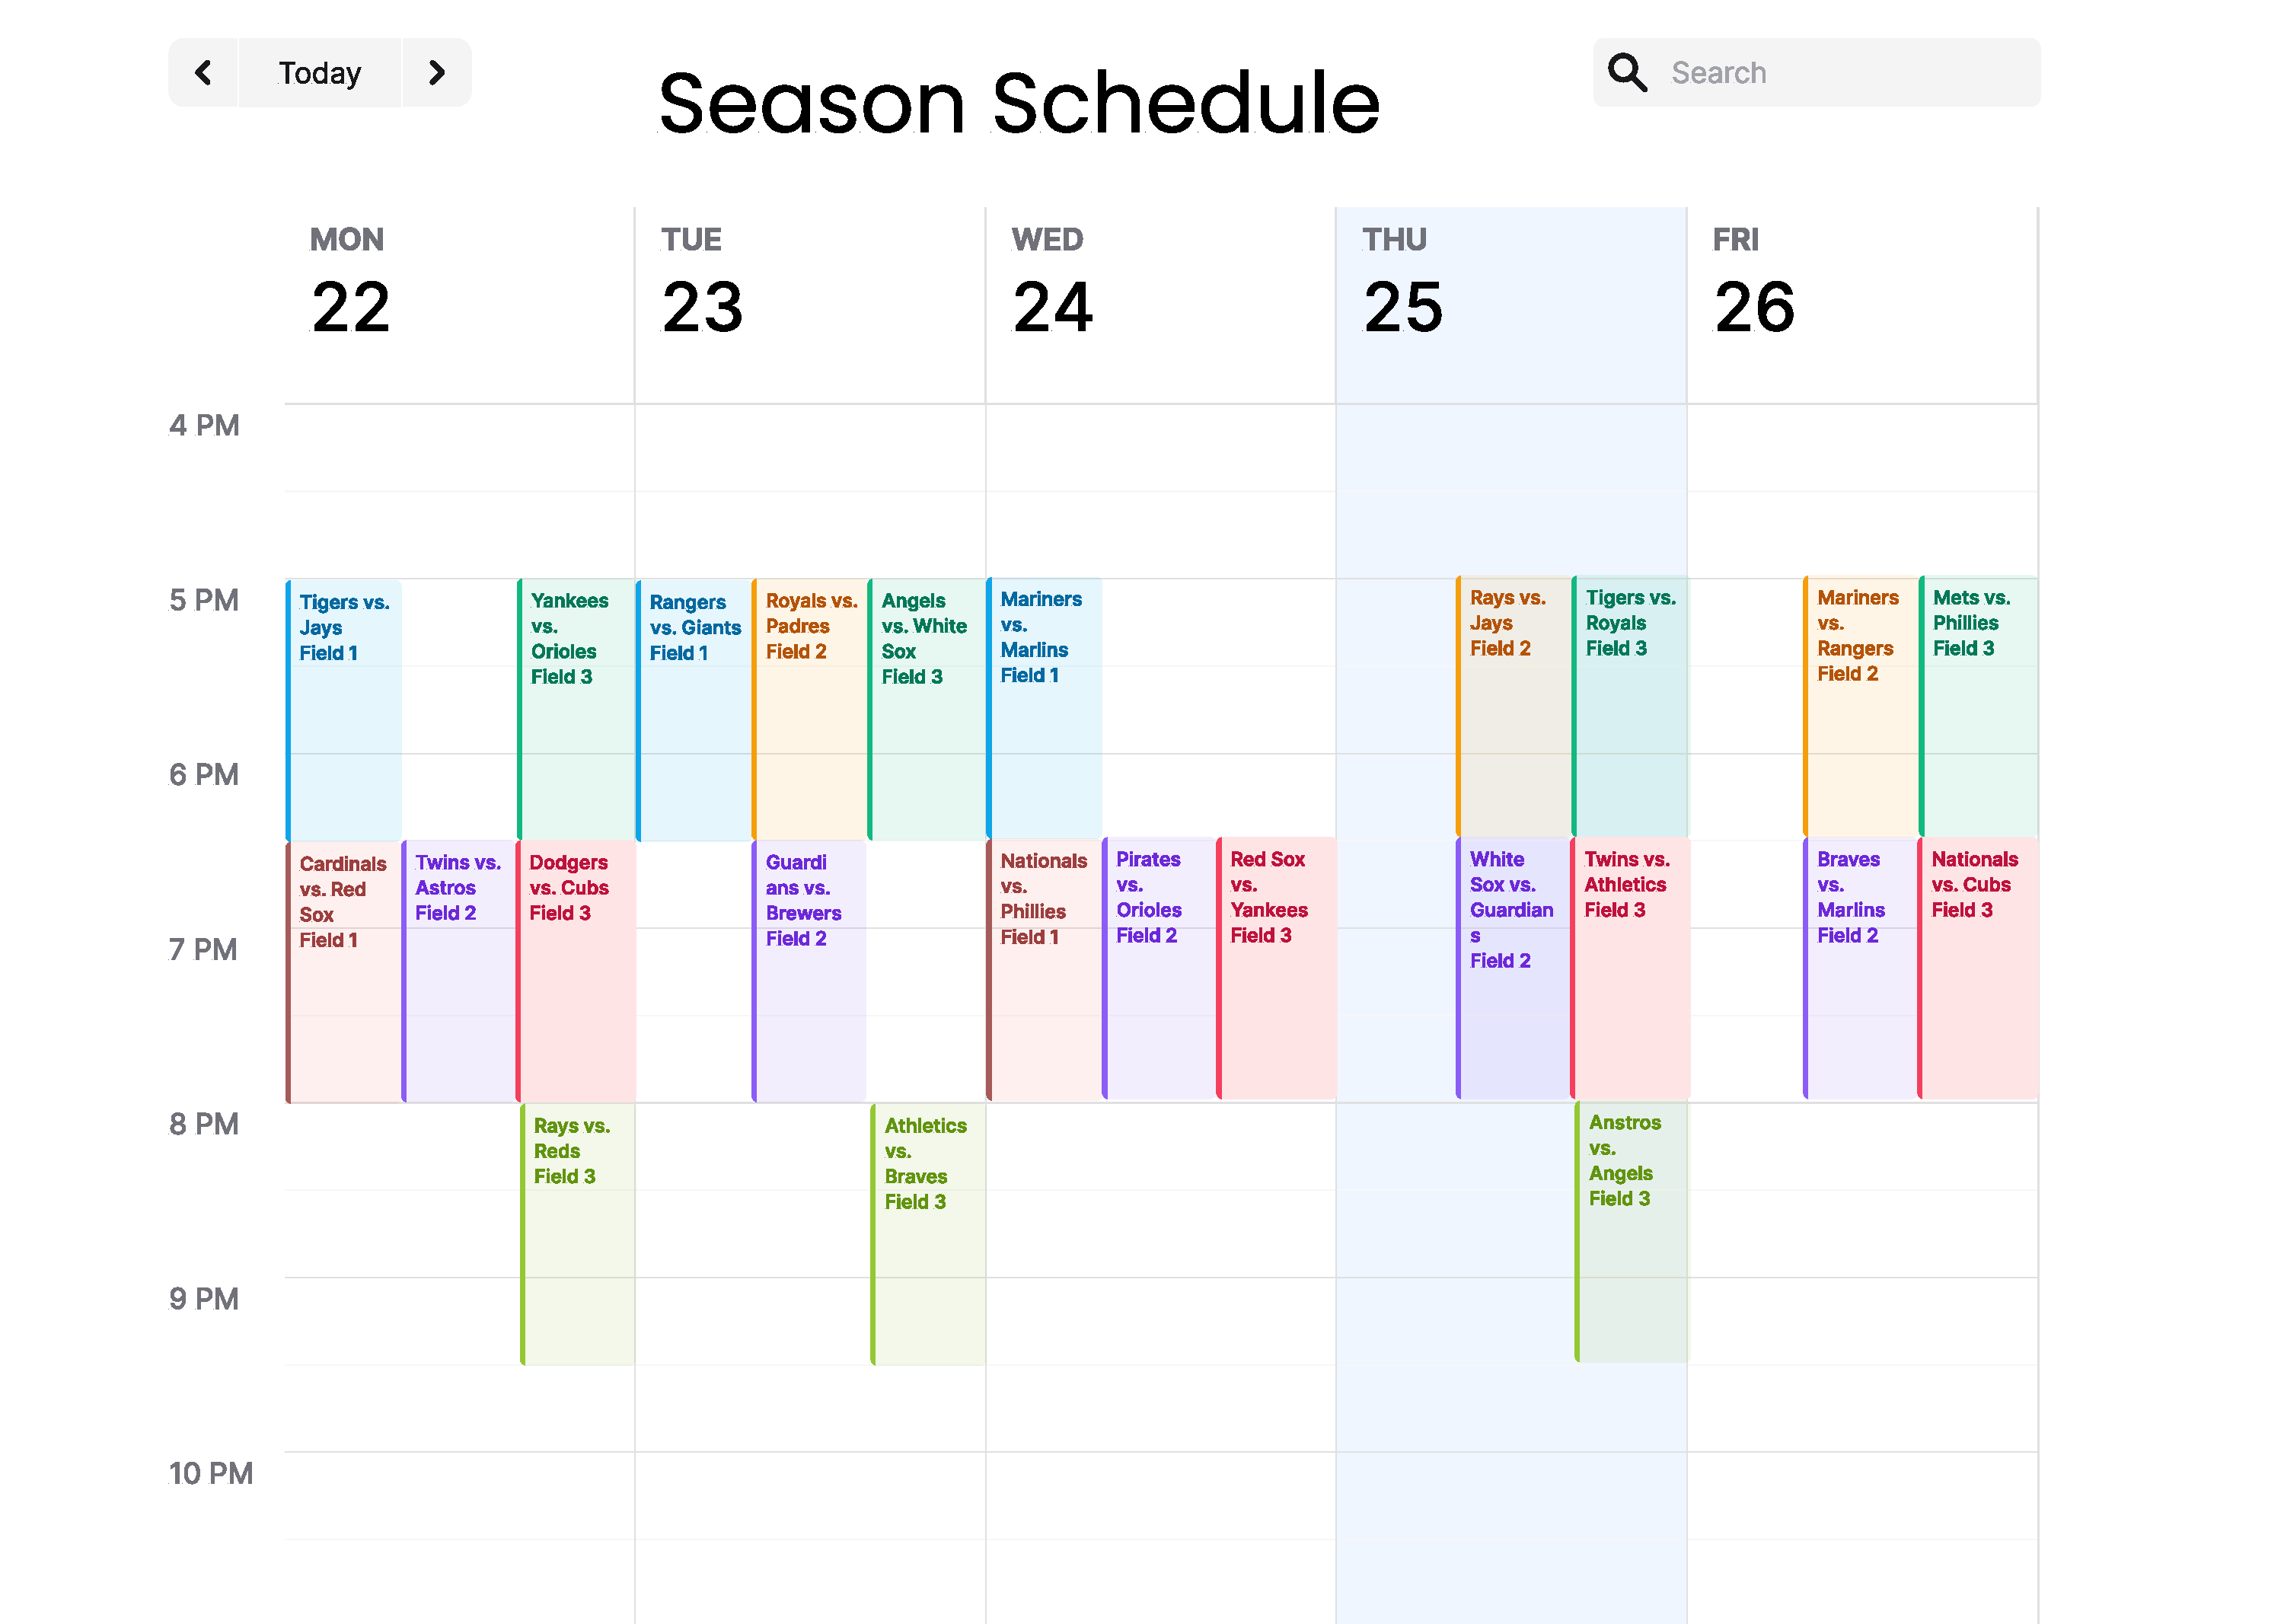
\includegraphics[scale=0.35]{Season Schedule.pdf}
\begin{figure}[H]
\centering
\caption{User interface: Season schedule page}
\label{FigSS}
\end{figure}

\centering
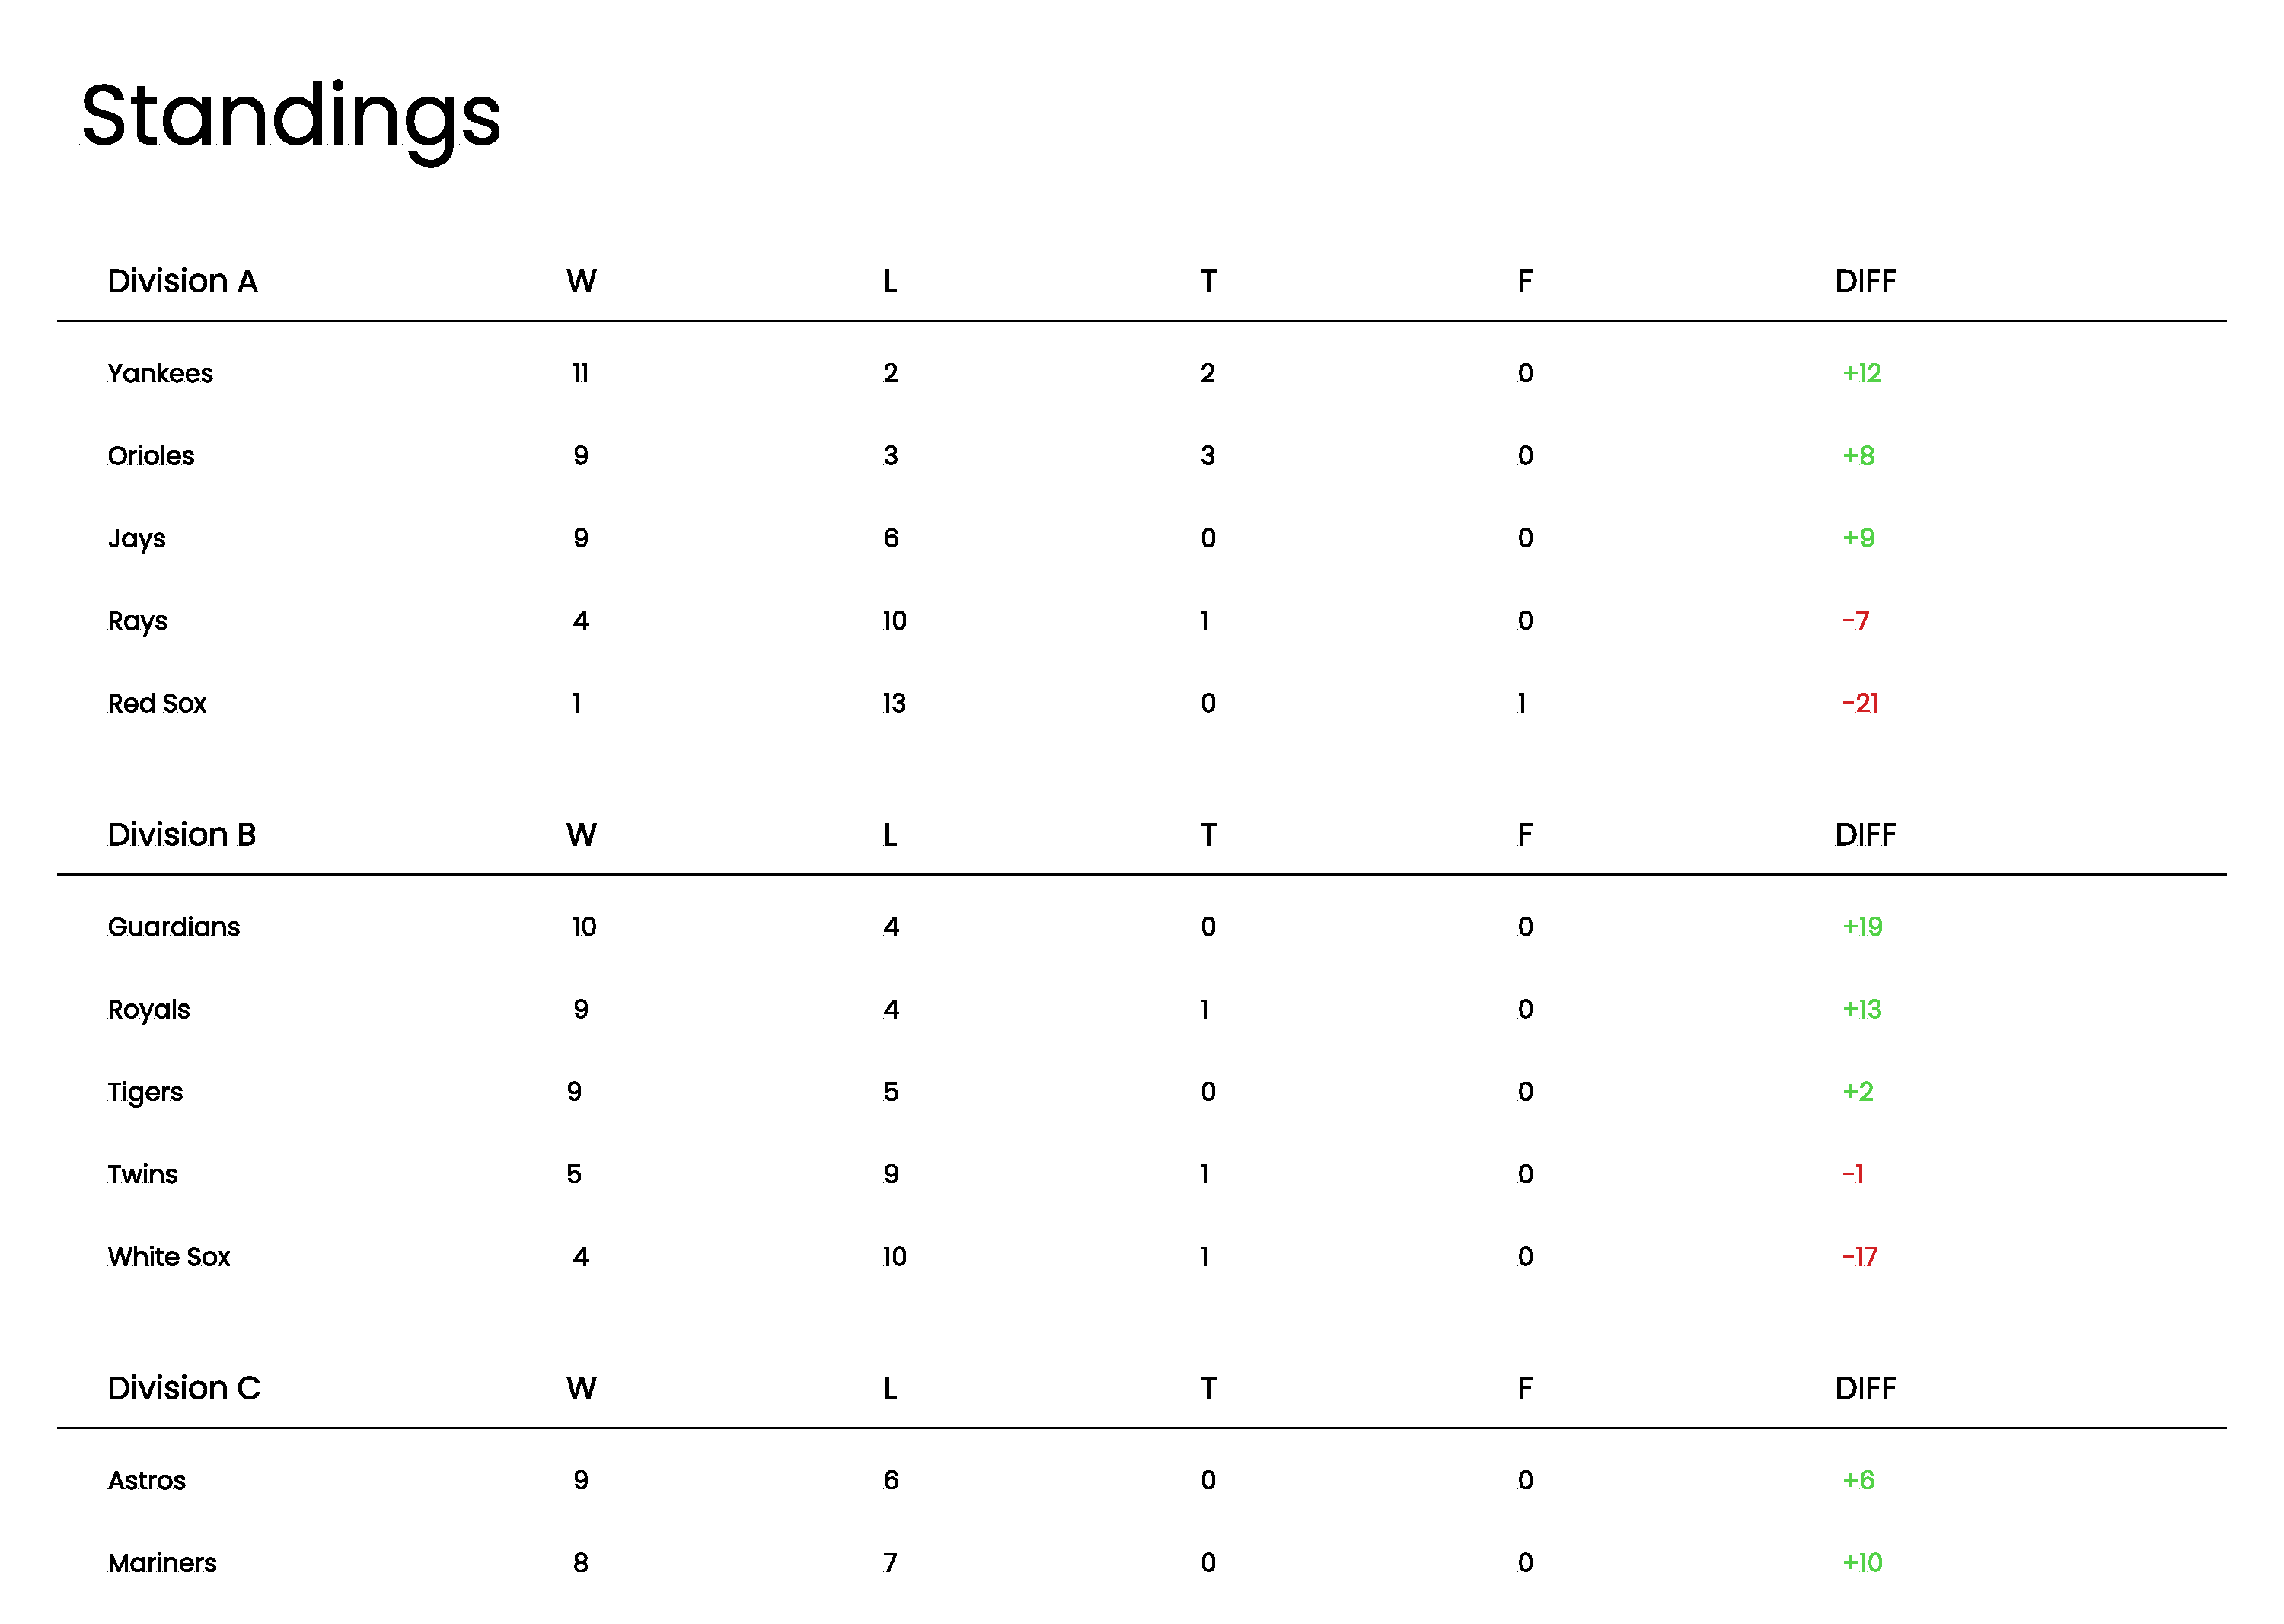
\includegraphics[scale=0.35]{Standings.pdf}
\begin{figure}[H]
\centering
\caption{User interface: League standings page}
\label{FigSS}
\end{figure}

\centering
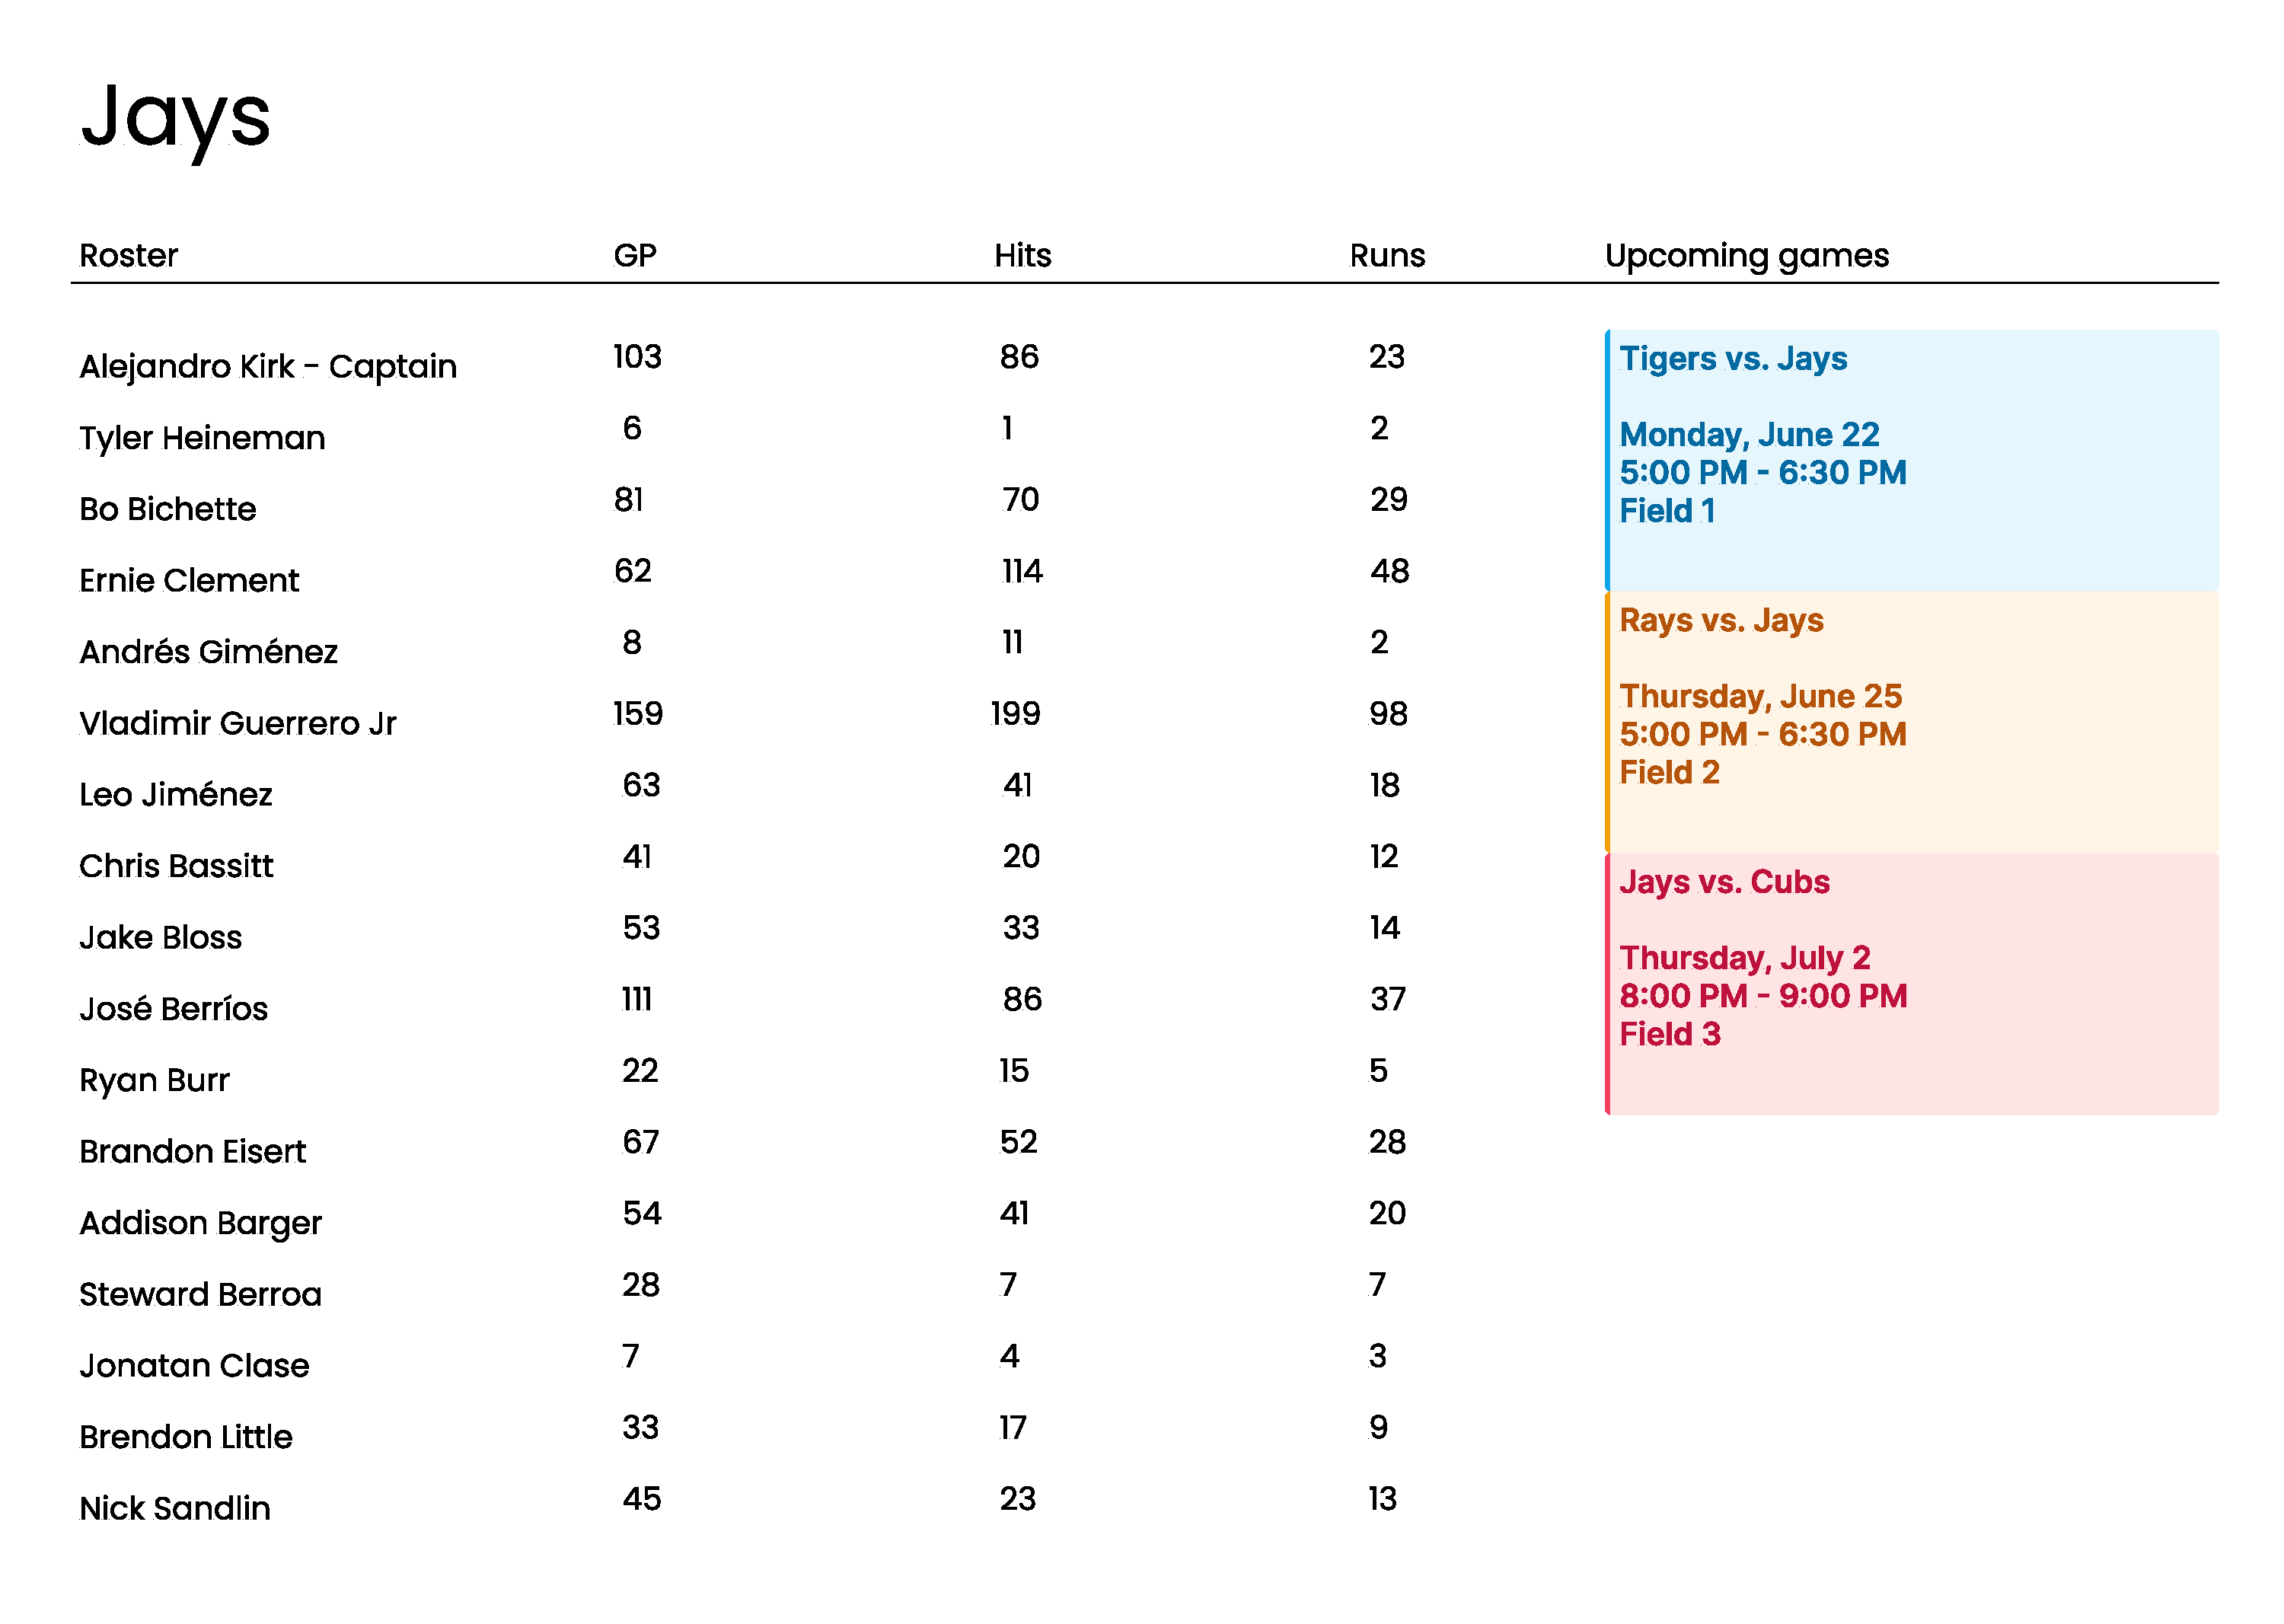
\includegraphics[scale=0.35]{Team Page.pdf}
\begin{figure}[H]
\centering
\caption{User interface: Team page}
\label{FigSS}
\end{figure}

\centering
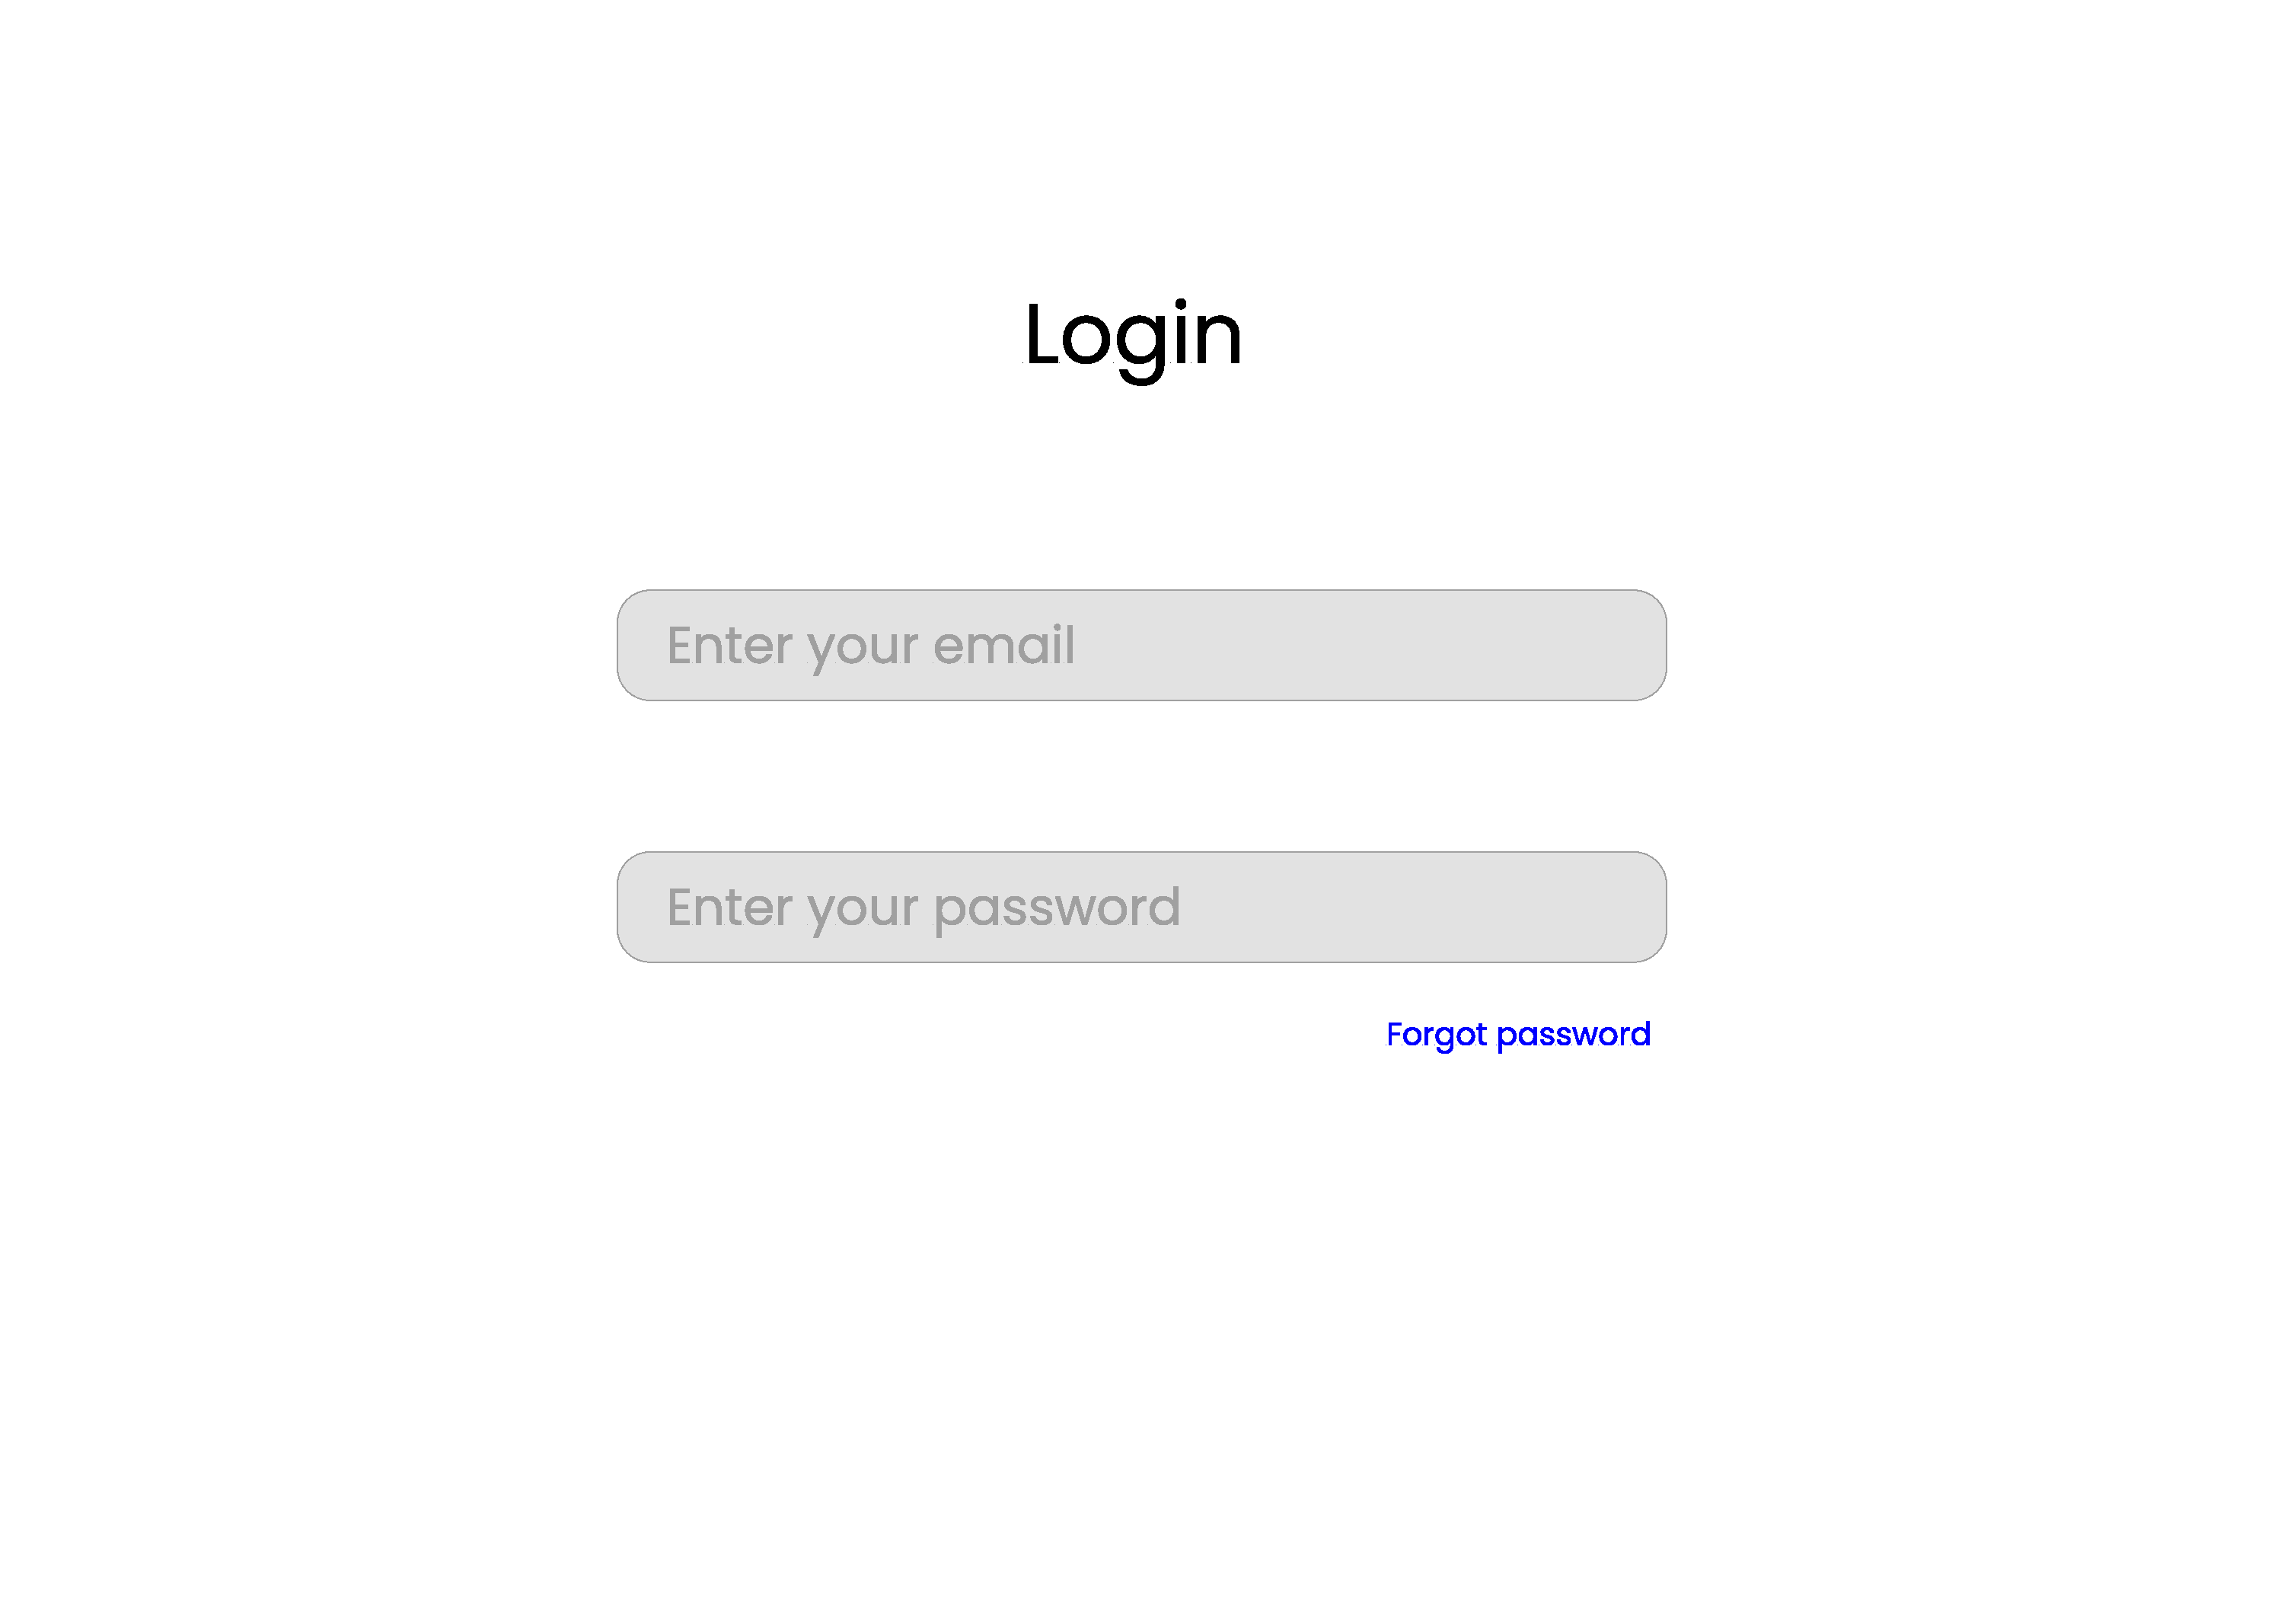
\includegraphics[scale=0.35]{Login.pdf}
\begin{figure}[H]
\centering
\caption{User interface: User log in page}
\label{FigSS}
\end{figure}

\end{document}